\chapter{Data}\label{chapter:data}
Dieses Kapitel beinhaltet Informationen über die Datensets. Auch erklären wir hier unsere Vorgehensweise, wie wir von den Rohdaten zu unseren "Trainingsdaten"(todo Begriffe abstimmen) kommen. For the following experiments we used two datasets: The OpenSubtitle dataset includes move subtitles, so this dataset represents spoken language. On the other hand we have the Reddit Submission Corpus dataset which contains written language. We choose those movie related datasets because we focus all subject about movies and films.

\section{Original datasets}
In diesem Abschnitt befinden sich Informationen zu den rohen Datensets. In the table \ref{table_data-origin} you can see some general information about the datasets.
\paragraph{OpenSubtitle} For each movie there exists a file which contains the movies subtitles in chronologically order. You can see en example in the picture \ref{?}.
\begin{table}[H]
	\centering
	\small
	\begin{adjustbox}{max width=\textwidth}
	\begin{tabular}{llllll}
		\toprule
		&  \specialcell{\emph{short name}}
		&  \specialcell{\emph{size} \\\textit{[GB]}}
		&  \specialcell{\emph{lines} \\\textit{[million]}}
		&  \specialcell{\emph{data format}}
		&  \specialcell{\emph{source}} \\
		\midrule
		\emph{OpenSubtitle 2016}						&OpenSubtitle	& 93	& 338	& XML	& \cite{lison2016opensubtitles2016}	\\
		\emph{Reddit Submission Corpus 2006-2015} 		&Reddit	&885	& 1'650	& JSON	&  Reddit Comments Corpus \protect\footnotemark \\
		\bottomrule
	
	\end{tabular}
	\end{adjustbox}
	\caption{Origing and some general information about the Datasets.}
	\label{tbl:data:rawData}
\end{table}
\footnotetext{$https://archive.org/details/2015_reddit_comments_corpus.$}
\section{Preprocessing}
In diesem Abschnitt wird erklärt, wie wir die Daten für das Training entsprechend extrahieren, filtern und anschliessend die Dialoge zusammengebaut werden.
\subsection{Extraction}
Was die erlaubten Zeichen betrifft, so gelten für beide Datensaätze die gleichen folgenden Regelen:
\begin{itemize}
	\item Gültige Zeichen sind a-z, A-Z, 0-9 und die Satzzeichen .,!?
	\item Wörter welche ungültige Zeichen beinhalten werden entfernt
	\item Zwischen Wörter und Satzzeichen wird immer ein Leerzeichen eingefügt
\end{itemize}
\paragraph{OpenSubtitle} Die Daten liegen sortiert nach Film Genre und Jahr vor. In diesen Unterordner befindet sich pro Film eine Datei welche im XML Format den Untertitel beinhaltet.
In einem ersten Schritt werden die gezippten Files in den Unterordner gesucht. Anschliessend wird jedes File entzippt und mit Hilfe der XML Library eingelesen. In der Abbildung \ref{?} ist ersichtlich, dass die einzelne Kinder des XML Objekts die Wörter enthalten. Die Wörter werden ausgelesen und entsprechend zu einem Satz kombiniert. Im der Abbildung \ref{?} sehen Sie den oben gezeigten Beispielsatz nach dem Preprocessing. Ein Dialog wiederum wir aus zwei nacheinander folgenden Sätzen erstellt.
\paragraph{Reddit Submission Corpus 2006-2015} Die Reddit Daten sind nach Jahr und Monat sortiert. Pro Monat gibt es eine Datei mit chronologisch aufsteigend sortierten JSON Objekten.
Als erstes werden, abhängig von den Programmierter, die Dateien pro gewünschtes Jahr zusammengesucht. Anschliessend werden diese Dateien aufsteigend mit Hilfe der JSON Library ausgelesen und nach entsprechenden Subreddits gefiltert. Ein Beispieleintrag finden Sie in der Abbildung \ref{?}. Da wir ein Dialog System mit Fokus auf Filme erstellen möchten, filterten wir die Daten entsprechend nach den Subreddit Tags, Movies, Films und Television. Nach dem Filtern der Daten, muss die Ursprüngliche Struktur der Kommentare wiederhergestellt werden. Für diesen Vorgang sind die Tags, $Parent_id$, $Link_id$ und Name relevant. Auf der obersten Kommentarebene ist die $Parent_id$ gleich der $Link_id$. Wobei beim ersten Vorkommnis pro ID ein neuer Beitrag beginnt. Für die Kinder eines Kommentars verhält es sich so, dass deren $Parent_id$ gleich dem Name Tag des Elternkommentar ist. Mit Hilfe der Shelve Library werden so die Urpsrünglichen Kommentarstrukturen erstellt. Dialoge werden generiert, indem der Elternknoten jeweils mit allen direkten Kindern kombiniert wird. In der Abbildung \ref{fig:data:reddit:utterance:construction} befindet sich ein theoretisches Beispiel. Es würden folgenden Kombinationen entstehen AB, AC, AD, DE und DF. Zwischen zwei Aussagen befindet sich jeweils unser Trennzeichen ('<<<<<END-CONV>>>>>'), welches während dem Training das Ende einer Konversation bedeutet.
\begin{figure}[h]
	\centering
	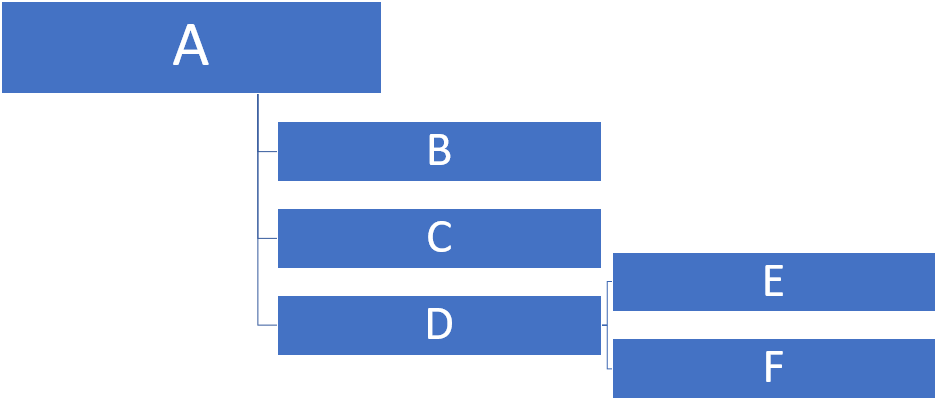
\includegraphics[width=10cm]{img/reddit_utterance_construction.PNG}
	\caption{Beispiel Reddit Aufbau der Trainingsdaten.}
	\label{fig:data:reddit:utterance:construction}
\end{figure}
Pro Datensatz erhalten wir nach dem Preprocessing eine Datei, welche pro Zeile eine Aussage enthält.
todo: Clique Bildung in text einbauen? entscheid für subreddit tags Visualisierung der CLique gemäss BigQuery
\section{Generate Vocabulary and a train, valid and text Dataset}
Die Spalte unique amount words in der Tabelle \ref{tbl:data:split:corpus:analyze} beinhaltet die Anzahl verschiedener Wörter pro Datensatz. Der OpenSubtitle besitzt 2.3 Millionen verschiedene Wörter und Reddit 3.1 Millionen. Da wir die Wörter nicht normalisieren können, müssen wir die zur Verfügung stehenden Wörter begrenzen. Ansonsten würde bei der Softmax Berechnung zu wenig Speicher zur Verfügung stehen(Genauer erklären, Referenz auf Kapitel wo erklärt wird). Dementsprechend wird das Vokabular spezifisch für jeden Datensatz generiert.
Dabei werden zuerst alle vorkommenden Wörter gezählt und nach der Häufigkeit absteigend ausgegeben. Wir extrahierten daraus 3 Vokabular, mit den jeweils 25k, 50k und 100k häufigsten Wörter. Die anschliessende Analyse zeigt die Abdeckung des Datensatzes pro Vokabular. Die Ergebnisse sind in der Tabelle \ref{tbl:data:split:corpus:analyze} ersichtlich. Wir sehen hier, dass die Abdeckung über den jeweiligen Dantesatz  mit allen 3 Vokabulargrössen ausreichend wäre.
Wir möchten die Abdeckung nun auf Aussage Ebene untersuchen. Dazu analysierten wir wie oft Wörter pro Aussage nicht erkannt werden. Die Graphen in der Abbildung \ref{fig:data:reddit:vocab:analyze} und \ref{fig:data:opus:vocab:analyze} weisen pro Datensatz ein leicht unterschiedliches Verhalten auf. Der Reddit Datensatz kann mit den 3 Vokabularen deutlich besser abgedeckt werden, als der Opensubtitle. Dies deuted darauf hin, dass die Häufigkeiten der Wörter im Opensubtitle näher beieinander sind, als diejenigen im Reddit Datensatz.
Todo: Könnte man noch untersuchen, Schnitt berechnen und dann Abweichung pro Wort berechnen. Wenn dieser Wert kleiner ist  => Theorie bestätigt.

Wir sehen also, dass trotz der grossen Anzahl Wörter (Angabe Wörter insgesamt pro Dataset), können bereits mit 50k Wörter \% der Wörter abgedeckt werden.

\begin{table}[H]
	\begin{adjustbox}{max width=\textwidth}
		\centering
		\small
		\begin{tabular}{lllllll}
			\toprule
			&  \specialcell{\emph{vocab size}	\\\textit{[thousand]}}
			&  \specialcell{\emph{total amount words}	\\\textit{[thousand]}}
			&  \specialcell{\emph{known words amount}\\\emph{words} \\\textit{[thousand]}}
			&  \specialcell{\emph{known words percent} \\\textit{[\%]}}
			&  \specialcell{\emph{unknown words amount}\\\emph{per utterance} \\\textit{[thousand]}}
			&  \specialcell{\emph{unknown words percent}\\\emph{per utterance} \\\textit{[\%]}}\\
			\midrule
			\emph{OpenSubtitle}	&25		&2362	&2096	&88.73	&266	&11.27\\
								&50		&2362	&2116	&89.57	&246	&10.43\\
								&100	&2362	&2127	&90.03	&236	&9.97\\
			\emph{Reddit}		&25		&1717	&1683	&98.00	&34		&2.00\\
								&50		&1717	&1699	&98.98	&17		&1.02\\
								&100	&1717	&1707	&99.42	&10		&0.58\\
			\bottomrule
		\end{tabular}
	\end{adjustbox}
	\caption{Abdeckung der Wörter pro Vokabulargrösse und Datensatz.}
	\label{tbl:data:split:corpus:analyze}
\end{table}

\begin{figure}[!htb]
	\minipage{0.5\textwidth}
	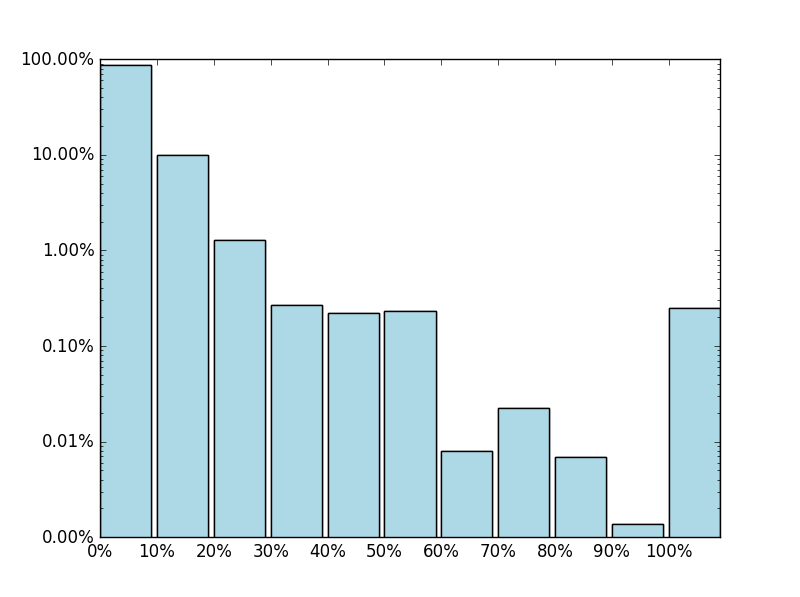
\includegraphics[width=\linewidth]{img/reddit_vocab_analyze_100k_perc.PNG}
	\centering
	\small
	\text{Reddit 100k}
	\endminipage\hfill
	\minipage{0.5\textwidth}
	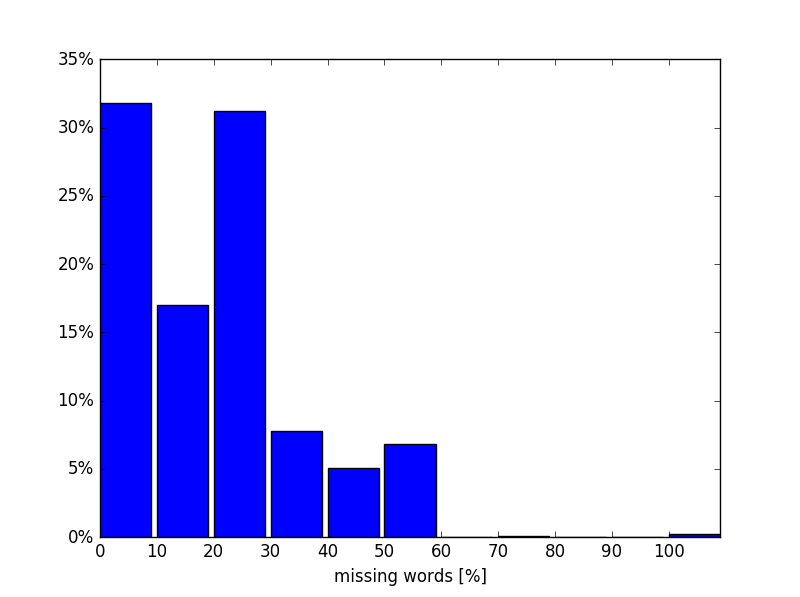
\includegraphics[width=\linewidth]{img/opus_vocab_analyze_100k_perc.PNG}
	\centering
	\small
	\text{OpenSubtitle 100k}
	\endminipage\hfill
	\minipage{0.5\textwidth}
	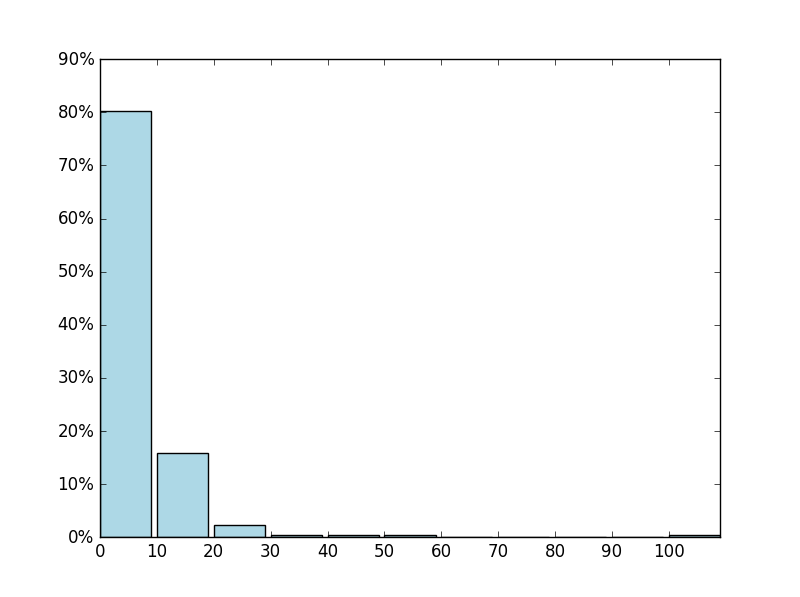
\includegraphics[width=\linewidth]{img/reddit_vocab_analyze_50k_perc.PNG}
	\centering
	\small
	\text{Reddit 50k}
	\endminipage\hfill
	\minipage{0.5\textwidth}
	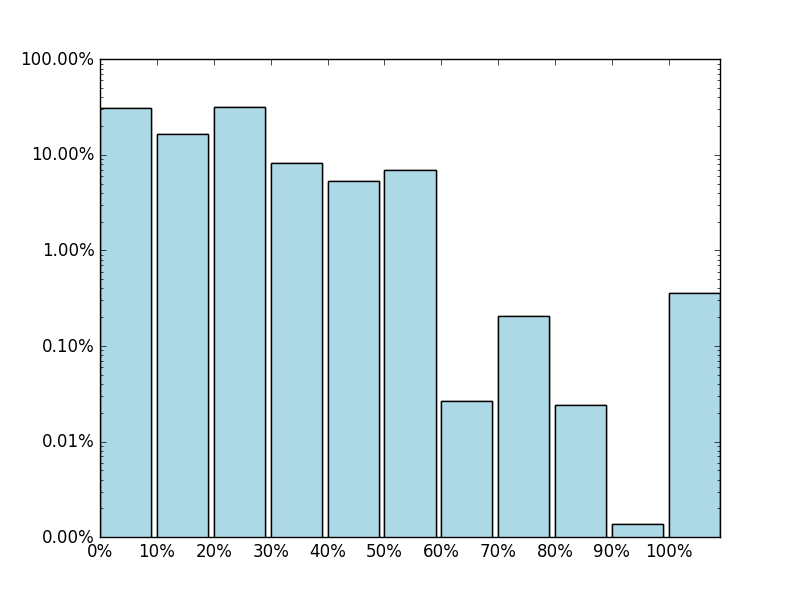
\includegraphics[width=\linewidth]{img/opus_vocab_analyze_50k_perc.PNG}
	\centering
	\small
	\text{OpenSubtitle 50k}
	\endminipage\hfill
	\minipage{0.5\textwidth}%
	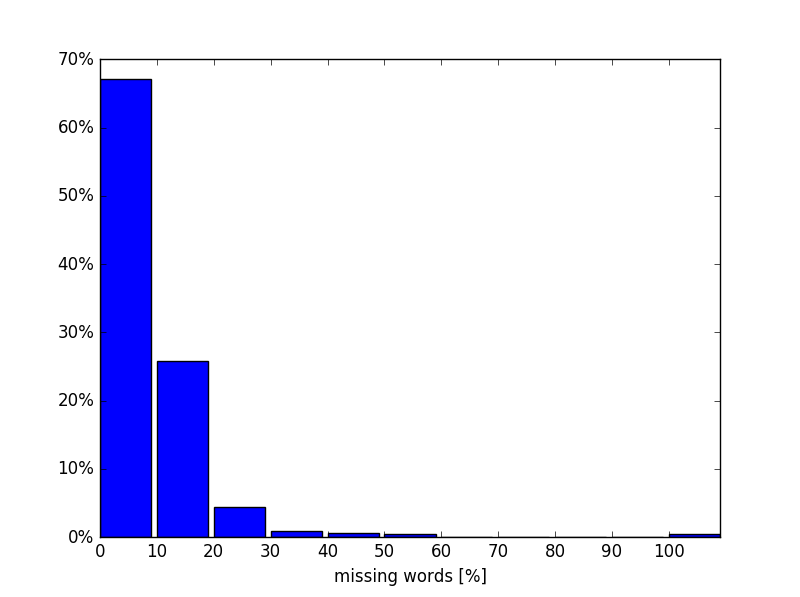
\includegraphics[width=\linewidth]{img/reddit_vocab_analyze_25k_perc.PNG}
	\centering
	\small
	\text{Reddit 25k}
	\endminipage\hfill
	\minipage{0.5\textwidth}%
	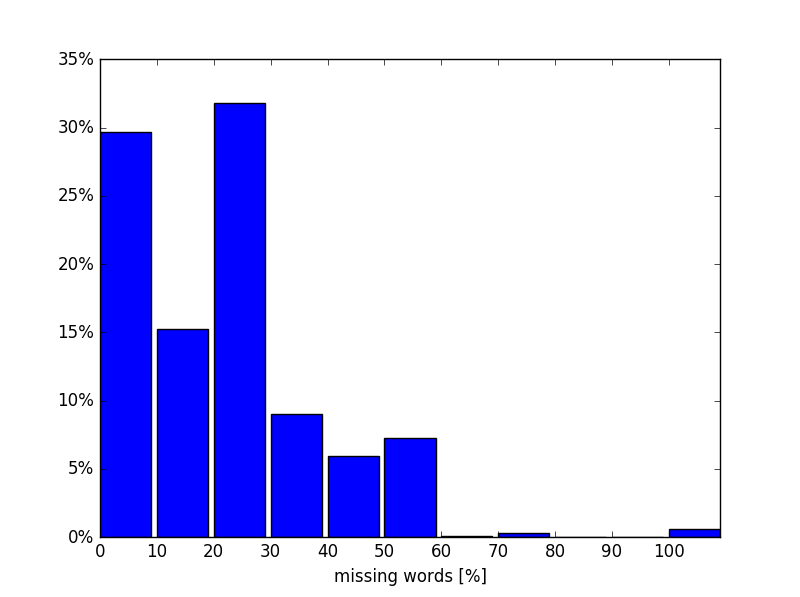
\includegraphics[width=\linewidth]{img/opus_vocab_analyze_25k_perc.PNG}
	\centering
	\small
	\text{OpenSubtitle 25k}
	\endminipage
	\caption{Die X-Achse steht für den Prozentsatz fehlender Wörter pro Aussage. Die Y-Achse entspricht der relativen Anzahl zum jeweiligen gesamten Datensatz.}
	\label{fig:data:reddit:vocab:analyze}
\end{figure}

Beim Durchsichten der Daten, empfanden wir die Qualität des OpenSubtitle Datensatzes als eher schlecht. Wir vermuteten die Ursache in der gesprochenen Sprache, da das Bild als wichtiger Informationsträger fehlt. Eine zusätzliche mögliche Begründung wäre es, dass die Bildszene endet und mit einigem zeitlichen Abstand erst wieder gesprochen wird. Somit würden Sätze kombiniert werden, welche nicht den gleichen Kontext besitzen. Deshalb haben wir die zeitlichen Abstände zwischen den Sätzen analysiert. Die Ergebnisse sind in der Grafik \ref{fig:data:analyse:timediff:opus} ersichtlich. Aufgrund der Ergebnisse, dass über 80\% der Aussagen in einem Zeitabstand kleiner gleich 5 Sekunden aufeinander folgen, verwerfen wir vorerst diese These als Ursache. In der Abbildung \ref{fig:data:analyse:timediff:opus} sind die Werte grösser 30\% auffällig hoch. Dies liegt einerseits an den Übergängen zwischen 2 Datensets und weil alle restlichen Werte in dieser Klasse landen. Dies sehen wir aber nicht als Problem an, weil über 80\% der Daten diese Problematik nicht betrifft.
Todo: erklären Wir unternehmen vorerst keine weiteren Schritte

\begin{figure}[h]
	\centering
	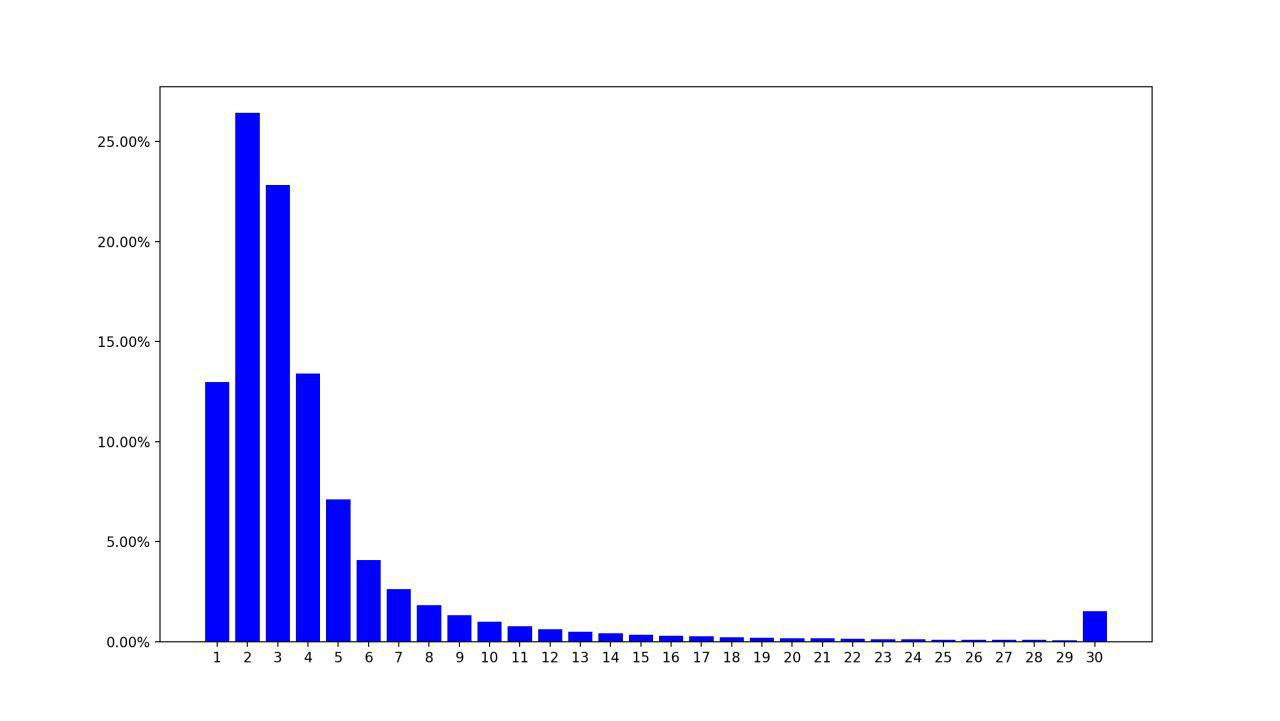
\includegraphics[width=15cm]{img/opus_time_analyze.PNG}
	\caption{Relative Verteilung der berechneten Zeiten (Diskret) in ganzen Sekunden zwischen zwei Äusserungen. Wobei die grössten Anteile die folgende 5 Zeitabstände haben: 13.0\% 1 Sekunde, 26.4\% 2 Sekunden, 22.8\% 3 Sekunden, 13.4\% 4 Sekunden und 7\% 5 Sekunden. Die resultierende Abdeckung dieser 5 häufigsten Zeitabstände beträgt 82.6\%.}
	\label{fig:data:analyse:timediff:opus}
\end{figure}

Wir untersuchten die Daten zusätzliche nach Häufigkeiten von Bi- und Trigrammen. Diese Vorgang war sehr rechenintensiv und dauerte entsprechend lange. Die Resultate sind pro Datensatz in den Abbildungen \ref{?} und \ref{?} ersichtlich. Das Ziel dieser Analyse ist es, die später generierten Sätze ebenfalls auf Bi- und Trigramme zu untersuchen um eine mögliche Korrelation auf der Ebene Phrase zu finden.
Todo: Wolkenbildung...
Bi-Gram Tri-Gram Analyse entweder mit WOlke, oder heat mat, tree map
Vielleicht gibt es noch eine andere Variante um dies darzustellen (besser), wenn möglich mit paper referenz
$http://infosthetics.com/archives/2006/03/subject_tag_news_heat_map.html$
$https://www.quora.com/What-are-alternatives-to-tag-clouds-for-information-visualization$


Schlussendlich teilten wir die Datensätze auf wobei 97\% als Trainingsdaten, 2\% als Validierungsdaten und 1\% als Testdaten verwendet werden. Die genauen Zahlen befinden sich in der Tabelle \ref{tbl:data:split:corpus}. Die Ursprünglichen Dialoge wurden dabei nur als ganzes aufgeteilt. Die zwei Aussagen des gleichen Dialogs blieben dementsprechend zusammen.
\begin{table}[]
	\centering
	\begin{adjustbox}{max width=\textwidth}
		\centering
		\small
		\begin{tabular}{lllll}
			\toprule
			&  \specialcell{\emph{set}}
			&  \specialcell{\emph{Percent from total} \\\textit{[\%]}}
			&  \specialcell{\emph{size} \\\textit{[MB]}}
			&  \specialcell{\emph{lines} \\\textit{[thousend]}}\\
			\midrule
			\emph{OpenSubtitle}		&train	&97	&9'393	&321'643	\\
									&valid	&1	&97		&3'315	\\
									&test	&2	&194	&6'631	\\
			\emph{Reddit}			&train	&97	&8'455	&75'297	\\
									&valid	&2	&185	&1'552	\\
									&test	&1	&92		&776	\\
			\bottomrule
		\end{tabular}
	\end{adjustbox}
	\caption{In this table you can see the resulting 3 sets per Dataset....}
	\label{tbl:data:split:corpus}
\end{table}

todo: paper relevant? $https://www.researchgate.net/publication/283986649_LSTM-based_Deep_Learning_Models_for_Non-factoid_Answer_Selection$
